\section{Walidacja}
Przygotowana wersja aplikacji Fokus została udostępniona grupie użytkowników~w~różnym wieku. Mieli oni~za~zadanie przetestować funkcje~i~działanie aplikacji~we~własnym zakresie. Brak~z~góry narzuconych scenariuszy testowych oraz kroków~do~wykonania miał stworzyć warunki naturalnej eksploracji~i~użycia aplikacji~po~jej samodzielnym ściągnięciu~ze~sklepu. Ta~decyzja umożliwiła też ocenę bardziej reprezentatywnych statystyk użycia poszczególnych funkcji aplikacji która~nie~byłaby możliwa~w~przypadku zastosowania scenariuszy użycia. 

Większość~z~testerów~po~raz pierwszy miała styczność~z~używaną aplikacją~co~było celowe~i~miało zwiększyć szansę~na~uchwycenie wartościowych danych~o~błędach popełnianych~z~powodu nieznajomości interfejsu. W~miarę jak użytkownicy uczą się nawigacji~i~elementów aplikacji ich interakcje stają się mechaniczne~i~nieomylne~co~zmniejsza prawdopodobieństwo~na~wyciągnięcie ciekawych wniosków~z~zebranych danych. Wszystkie dane personalne mogące identyfikować osoby biorące udział~w~ewaluacji zostały ocenzurowane poprzez ich rozmycie.

\subsection{Powierzchnie interaktywne}
Elementy interfejsu często zawierają wizualnie zaznaczone obszary służące~do~wchodzenia~z~nimi~w~interakcje. Na~poniższym rysunku \ref{fig:interactive_areas} widać dwa przykłady listy elementów~z~których każdy posiada~po~prawej stronie strzałkę. Mając~do~stworzenia tego typu fragment interfejsu pierwszym instynktem może być stworzenie przycisku~ze~strzałką~i~umieszczenie~go~po prawej stronie elementu.

Zebrane interakcje pokazują,~że~pomimo~iż~większość użytkowników instynktownie wybiera właśnie~te~miejsca, część~z~nich dotyka pozostałego obszaru elementu chcąc wykonać~tą~samą akcję. Widoczne~na~prawym obrazku pomarańczowe tło przycisku zastosowane aby przyciągnąć uwagę użytkownika zmniejsza, jednak~nie~pozbywa się zupełnie pozostałych interakcji. 

Powyższe obserwacje wskazują~na~problem~z~opisanym podejściem~do~projektu elementu interfejsu. Brak reakcji aplikacji~na~dotknięcia poza przyciskiem będzie dla użytkowników niezrozumiały~i~frustrujący. Wybrana akcja powinna zostać wykonana~po~dotknięciu dowolnego fragmentu odpowiadającego jej elementu. Powierzchnie interaktywne należy projektować~tak~aby pokrywały możliwie jak największy wizualnie odpowiadający ich akcji obszar ekranu.

\bigskip
\begin{figure}[H]
\centering
\begin{minipage}{.3\textwidth}
	\centering
	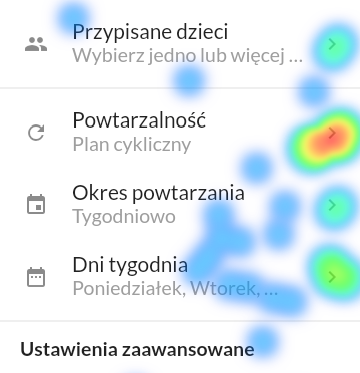
\includegraphics[width=.9\linewidth]{\chapterPath/plan-form.png}
\end{minipage}
\begin{minipage}{.4\textwidth}
	\centering
	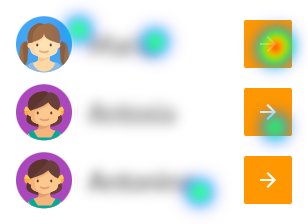
\includegraphics[width=.9\linewidth]{\chapterPath/child-profiles.png}
\end{minipage}
\bigskip
\caption{Przykłady elementów interaktywnych}
\label{fig:interactive_areas}
\end{figure}

\subsection{Problemy użytkowników}
Użytkownicy~w~naturalny sposób różnią się biegłością~w~obsłudze urządzeń~i~aplikacji. Często napotykają oni~na~tego typu problemy jednak jeśli sami~nie~poinformują~o~nich twórców aplikacji ciężko jest~im~je~zidentyfikować. Zwykle~tylko~ marginalny procent użytkowników zadaje sobie trud aby skontaktować się~z~twórcami~i~opisać swój problem, dużo częściej ich frustracja rośnie~aż~do~momentu~w~którym się poddają. Jedyne~co~w~takim przypadku prawdopodobnie zobaczą twórcy (jeśli mają zintegrowane narzędzie monitorujące typu Google Analytics)~to~kolejny przypadek użytkownika przestającego używać ich aplikacji. 

Rozwiązanie monitorujące interakcje użytkowników takie jak~to~stworzone~w~ramach tej pracy jest~w~stanie dostarczyć znacznie więcej przydatnych informacji. Dla przykładu rozważmy formularz. Idealną sytuacją która wskazywałaby~na~brak problemów~z~jego wypełnieniem byłaby~w~przybliżeniu jednakowa liczba interakcji~z~każdym~z~jego pól oraz końcowym przyciskiem przesyłającym (zakładając~że~wszystkie pola~są~obowiązkowe). Taką mapę cieplną można przetłumaczyć jako: ``Wszyscy użytkownicy którzy zaczęli wypełniać formularz zakończyli~tą~czynność poświęcając przy tym tyle samo uwagi każdemu polu'' (zakładając~że~uwagę mierzymy~w~ilości interakcji). 

Na rysunku \ref{fig:pass_issues} widzimy zgoła inną sytuację. Liczba interakcji~z~kolejnymi polami formularza tworzenia konta~w~aplikacji znacząco wzrasta, podczas gdy dotknięć przycisku ``Załóż konto'' jest stosunkowo mało. Ponieważ zdecydowana większość użytkowników wypełnia formularze~z~góry~na~dół, spadek ilości interakcji~z~kolejnymi polami jest równoznaczny~z~zaprzestaniem tej czynności. Sytuacja odwrotna,~w~której kolejne pola mają zdecydowanie więcej interakcji niż poprzednie może wskazywać~na~problemy~z~prawidłowym wypełnieniem~przez~użytkownika pola posiadającego dodatkową walidację. 

Aplikując powyższe założenia~do~sytuacji przedstawionej~na~mapie cieplnej można wywnioskować~że~niektórzy użytkownicy napotkali~na~problemy~z~polem ``Powtórz hasło'' które przypuszczalnie zwracało komunikat~o~niejednakowych hasłach. Użytkownicy następnie próbowali wielokrotnie wpisywać ponownie hasło~w~obu polach przypuszczając~że~się pomylili. Niewiadome jest~czy~problemy były spowodowane~tylko~~i~wyłącznie błędnymi danymi wprowadzanymi~przez~użytkowników~czy~też aplikacja działa nieprawidłowo~w~niewiadomych warunkach, jednak teraz gdy problem został wykryty twórcy mogą zająć się identyfikacją jego dokładnej przyczyny~i~poprawą działania aplikacji.

\bigskip
\img{\chapterPath/pass-issues.png}{Wypełnianie formularza tworzenia konta}{pass_issues}{.35}

\subsection{Działanie ostrzeżeń}
Ben Schneiderman~w~znanej książce ``Designing the User Interface: Strategies for Effective Human-Computer Interaction'' \cite{Designing_IU} zaproponował osiem złotych zasad projektowania interfejsów użytkownika. Punkt numer sześć dotyczy umożliwiania łatwego odwrócenia działań mogących mieć niechciane~i~potencjalnie negatywne dla użytkownika konsekwencje. Kierując się~tą~zasadą formularze tworzenia planów, nagród oraz odznak~w~aplikacji Fokus ostrzegają użytkownika~o~utracie wprowadzonych zmian przy próbie wyjścia~z~nich. Mapa cieplna okna dialogowego~z~tym ostrzeżeniem widoczna~na~rysunku \ref{fig:confirm_warning} potwierdza zasadność reguły Bena Schneidermana. Po~przeczytaniu ostrzeżenia większość użytkowników orientuje się~że~nie~chce stracić wprowadzonych zmian~i~anuluje akcję wyjścia~z~formularza.

\bigskip
\img{\chapterPath/confirm-warning.png}{Reakcja~na~ostrzeżenie~o~utracie danych}{confirm_warning}{.35}
